\documentclass{article}

\usepackage{graphicx} % Used to show UML model in eps
\usepackage{datetime} % Used to format time in LaTeX
\settimeformat{hhmmsstime} % The format we use for time 
\setlength{\parskip}{\baselineskip} % Put exactly one line between paragraphs
\setlength{\parindent}{0pt} % Do not indent paragraphs
\usepackage{hyperref} % Allows URLS to appear in the document

\begin{document}
\title{TBA Gate Model Assignment}
\author{Joris Slob}
\date{October 2014}
\maketitle

\section{Introduction}

For a job application at TBA, I was given an exercise to show my
technical skills. The precise description of the exercise can be found
in ASSIGNMENT.md. In this report, I will describe my general approach
to this exercise.

\section{Estimation on paper}

To determine the approach I would take I first did some simple
calculations to see what I could expect. For this I took the xlsx file
and made a quick estimate of the solution.

An important observation is that the entries in the xlsx file are all
for one day. The first truck arrives at the harbor at $T_1 =
\mbox{\formattime{6}{2}{29}}$ and the last truck arrives at $T_{1327}
= \mbox{\formattime{15}{24}{16}}$. That means that 1327 trucks arrive
in 561.78 minutes for an average of 2.36 trucks/min.

To deal with this load every part of the harbor has to be able to deal
with this rate of trucks. An entry gate with one lane takes 3 minutes
on average to deal with a truck. To handle 2.36 trucks/min requires
$\frac{2.36}{1/3} = 7.08$ lanes.

A stack modules take 2 minutes on average to deal a truck and there
are ten, so they can handle 5 trucks/min. We expect no flow problems
in the stack modules.

The exit gate takes 1 minute on average to deal with a truck, so to
handle the 2.36 trucks/min requires 2.36 lanes.

Let us model this gate problem in software to verify these results.

\section{Software model}

\subsection{Overview}

The goal of the software is to simulate and find the optimal number of
entry and exit lanes. For speed and accuracy, I could reduce the
problem to the bare minimum that matters to this particular question
and simulate just that. The other extreme possibility is to make a
fully graphical simulator that shows the state of the harbor at every
second. I decided to go for the middle ground, which is an application
without a graphical interface, but design the application in such a
way that it is still possible to add one later.

This implementation of the gate simulation uses discrete timesteps. It
keeps track of all points in time when the location of a truck
changes. The Schedule class manages this information. The schedule in
the Schedule class is a datastructure that has an ordered list of time
objects associated with truck objects that will be active at that
time. In the TruckActivity file we can already see that there are
concurrent activities taking place. In this simulation we do not
handle them concurrently, because the trucks have no interaction with
eachother in this simulation. The SortedMap interface comes close to
our wishes, but it does not allow duplicate keys, so if we wanted to
use this, we would have to implement our datastructure as
SortedMap\textless LocalDateTime, List\textless ?\textgreater
\textgreater. Instead of creating this structure, I have reused the
TreeMultimap implementation from the Google Collections Library.

Trucks play a special role in this simulation. They represent both
physical trucks moving through the harbor and they are message objects
that facilitate communication between the Schedule, Component and
finally the Statistics classes.

The code is split up in three packages, components, simulator and
util. The simulator contains all the classes that are necessary to run
a simulator and report back on the statistics. The components package
contains all the seperate components of the harbor that trucks have to
go through. The util package contains two utility classes, one for
parsing the Excel file and one to deal with Gamma Distributions.

The class layout of the most important classes can be seen in the
following UML diagram.

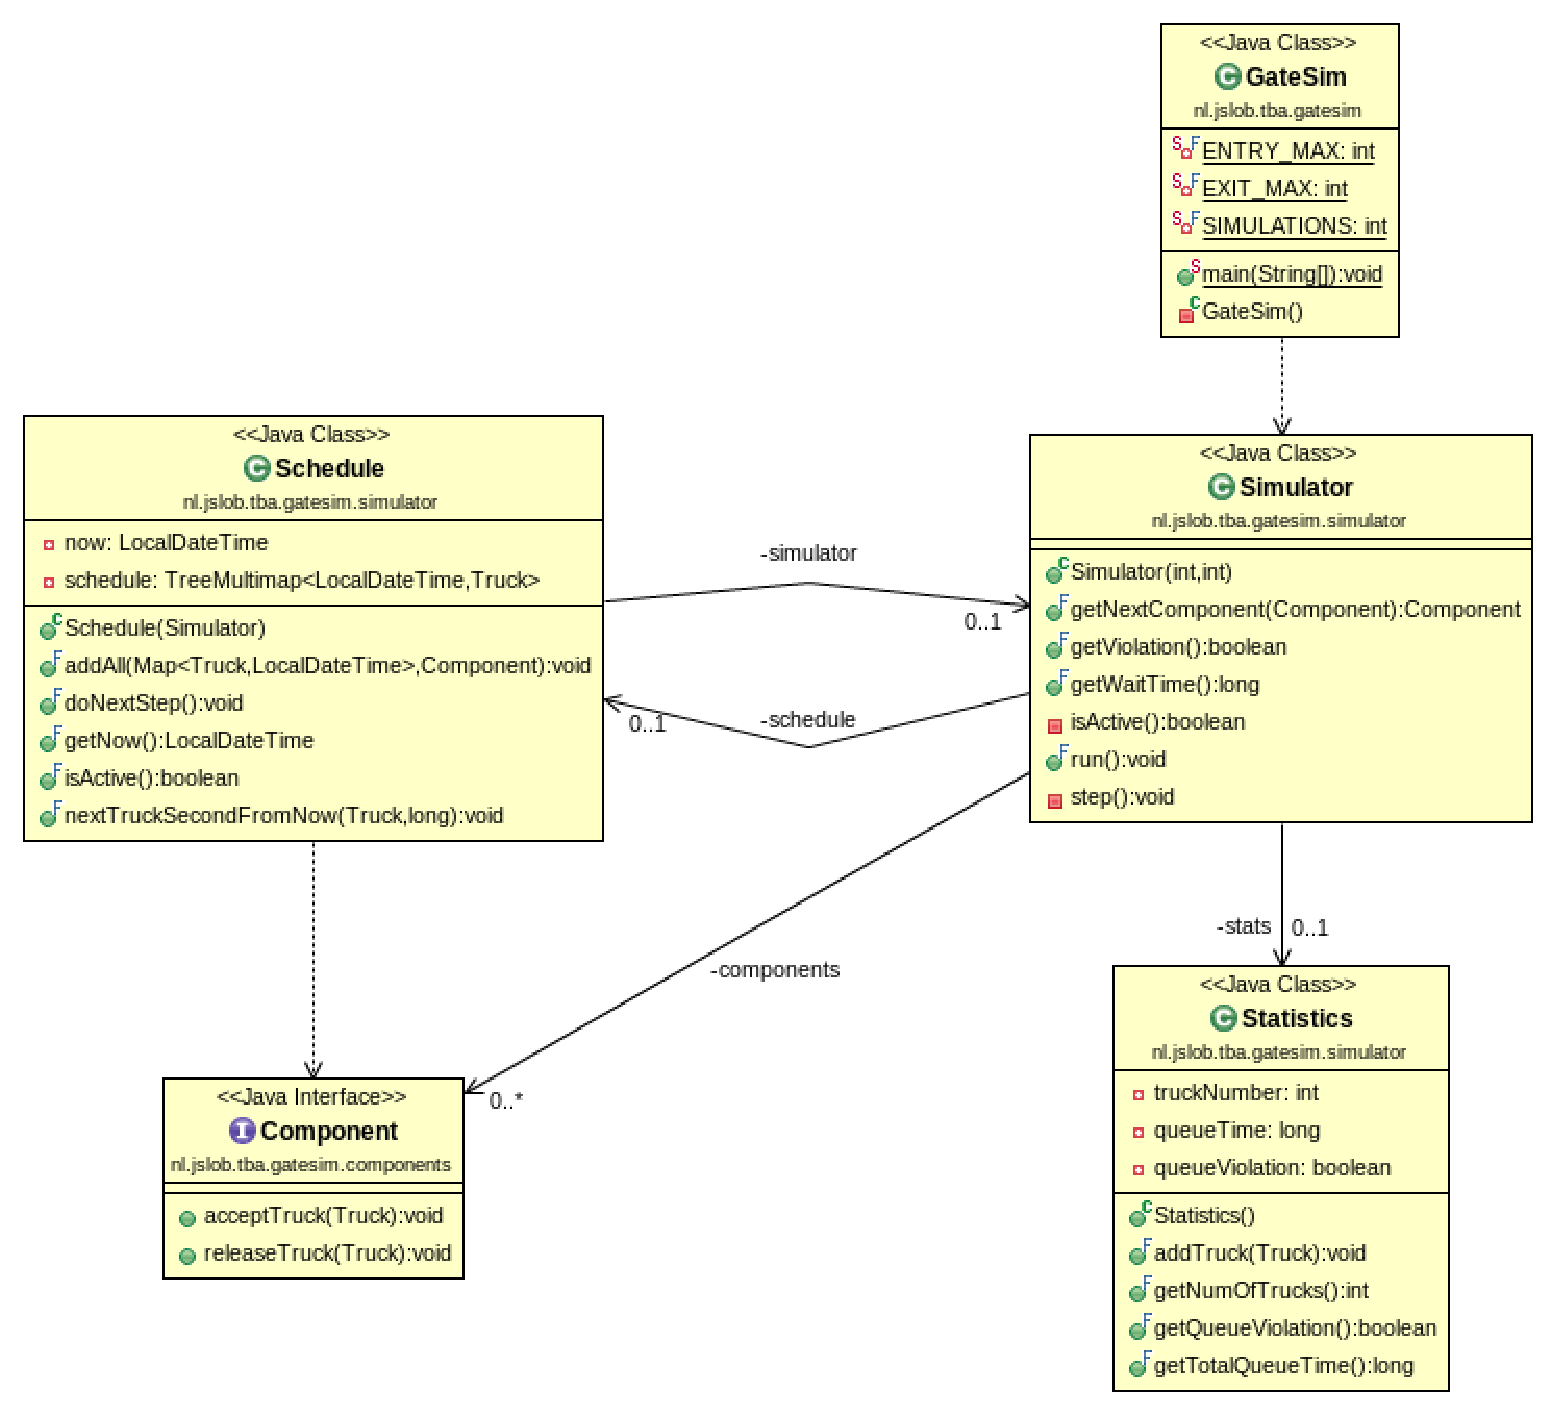
\includegraphics[scale=0.4]{Simulator.eps}

\subsection{Implementation}

The code is available on Github at:\\ 
\url{https://github.com/jorisslob/TBA_Assessment}\\ 
Github was chosen as an offsite code repository to allow work from
multiple computers and to have a backup of the code.

The Java Application was built using Apache Maven 3.0.5. This allows
other users to easily build and deploy the application. It also deals
with dependency management.

Our project has five dependencies on external libraries:

\begin{description}
\item[Apache POI] Needed to parse Excel files.
\item[Apache POI OOXML] Needed to parse the xlsx files specifically.
\item[Apache Commons Math3] Used for the Gamma Distribution.
\item[Google Guava Collections] Used for the TreeMultimap datastructure.
\item[JUnit] Used for test cases.
\end{description}

Code was written for JRE 8 in Eclipse Luna.

The test cases are not finished yet: they only cover part of the
GammaDistributionRate currently.

The output is now done to stdout, but could be adapted later. The
results were piped to a csv file and visualized using a gnuplot
script.

\section{Results}

The first result (with the smallest number of gates) that satisfies
the assignment (no queue greater than 30 trucks at any time) is the
model with 7 entry lanes and 3 exit lanes. This comes close to the
initial estimate given in the introduction. In this assignment we have
introduced another metric to evaluate the performance of the system:
TotalQueueTime. With data on the total time lost in queues the harbor
can consider opening more lanes to compensate truck waiting
time. Opening new lanes and operating them also has a cost, but these
were not given in the assignment. The graph shows the Total Queue Time
for different configurations of the harbor.

\includegraphics[scale=0.9]{results.eps}

\end{document}
